\documentclass{bmvc2k}

%% Enter your paper number here for the review copy
% \bmvcreviewcopy{??}

% Configuracao de linguagem do documento:
% portugues e ingles
\usepackage[brazilian]{babel}
\usepackage[utf8]{inputenc}
\usepackage{multirow}
\usepackage{xcolor}


\title{Exploração da Visão {Estéreo}}

% Enter the paper's authors in order
% \addauthor{Name}{email/homepage}{INSTITUTION_CODE}
\addauthor{Rodrigo Ferreira Guimarães}{rodrigofegui@unb.br}{1}

% Enter the institutions
% \addinstitution{Name\\Address}
\addinstitution{
  Departamento de Ciência da Comptutação\\
  Universidade de Brasília\\
  Campus Darcy Ribeiro, Asa Norte\\
  Brasília-DF, CEP 70910-900, Brazil,  
}

\runninghead{Guimarães, Rodrigo F.}{Exploração da Visão {Estéreo} -- \today}

% Any macro definitions you would like to include
% These are not defined in the style file, because they don't begin
% with \bmva, so they might conflict with the user's own macros.
% The \bmvaOneDot macro adds a full stop unless there is one in the
% % text already.
% \def\eg{\emph{e.g}\bmvaOneDot}
% \def\Eg{\emph{E.g}\bmvaOneDot}
% \def\etal{\emph{et al}\bmvaOneDot}

%-------------------------------------------------------------------------
% Document starts here
\begin{document}

\maketitle

\begin{abstract}
    A compreensão do mundo através da visão é um conceito intuitivo à humanidade, mas ao possibilitar isso às máquinas têm-se um extenso campo de pesquisa, a visão computacional. Ao se tratar da compreensão 3D do mundo é preciso recorrer as técnicas de visão estéreo e cálculo dos mapas de disparidade e de profundidade para os objetos de estudo para imagens correspondentes retificadas ou não. Este projeto visa a exploração e o entendimento sobre esses conceitos, com implementação em Python com uso da biblioteca~\emph{OpenCV}.
\end{abstract}

\section{Introdução}
    \label{sec:intro}
A percepção sobre o mundo é feita através dos sentidos, dentre eles existe a visão. Com ela a humanidade pode distinguir formas, padrões, luzes e sombras de estruturas 3D que a cerca. Ao possibilitar esta mesma interpretação ao computador têm-se a denominada~\emph{visão computacional}~\citep{Szeliski2012}. Esta área possui diversas aplicações, como:~\emph{autentificação visual},~\emph{geração de panorâmicas},~\emph{captura de movimentos},~\emph{vigilância},~\emph{modelagem 3D a partir de imagens} e tantas outras mais. Para os casos cujo objetivo é entender o mundo a partir das múltiplas imagens é preciso usar~\emph{visão estéreo}.

\subsection{Geometria}
    \label{subsec:intro_geo}
No sistema de coordenadas euclidianas há um problema da representatividade da origem e dos demais pontos, uma vez que o primeiro é um ponto distinto e os demais são geometricamente idênticos. Como solução têm-se as~\emph{coordenadas homogêneas}, onde a origem é removida do plano e acrescida de uma dimensão~\cite{Li2001}. Nestas coordenadas, têm-se as equivalências de representação: pontos 2D são representados como $\mathbf{X} = (x, y)$ no espaço euclidiano são representados como $\mathbf{\Tilde{X}} = \mathbf{\Tilde{w}}(x, y, 1)$; linha 2D de $\mathbf{L} = ax + by + c$ paraa $\mathbf{\Tilde{L}} = (a, b, c)$; e ponto 3D de $\mathbf{X} = (x, y, z)$ para $\mathbf{\Tilde{X}} = \mathbf{\Tilde{w}}(x, y, z, 1)$.

Em coordenadas homogêneas, as transformações geométricas são multiplicação de matrizes, como: a~\emph{translação} ($\mathbf{x}'_{trans} = \big[ ~\mathbf{I}  ~|~ \mathbf{t}~ \big] ~ \mathbf{\Tilde{x}}$) e a~\emph{rotação com translação} ($\mathbf{x}'_{rot + trans} = \big[ ~\mathbf{R}  ~|~ \mathbf{t}~ \big] ~ \mathbf{\Tilde{x}}$), onde $\mathbf{R}\mathbf{R}^{T} = \mathbf{I}$ e $| \mathbf{R} | = 1$.

Além disso, um produto vetorial $\mathbf{v}_{\times} = \mathbf{a} \times \mathbf{b}$ é equivalente à multiplicação de matrizes $\mathbf{v}_{\times} = {[\mathbf{a}]}_{\times} \mathbf{b}$, sendo ${[\mathbf{a}]}_{\times}$ a forma matricial do operador de produto vetorial~\cite{Szeliski2012}.

\subsection{Câmeras}
    \label{subsec:intro_cam}
Para a aquisição de imagens, uma câmera é posicionada no mundo com um ponto de referência
% , conforme ilustrado na Figura~\ref{fig:intro_cam_coord}
. Dessa forma, por semelhança de triângulos, a projeção $\mathbf{P}$ de pontos 3D do mundo em pontos 2D da imagem corresponde a $(x, y, z) \to (f \frac{X}{Z}, f \frac{Y}{Z}, f) = (f \frac{X}{Z}, f \frac{Y}{Z})$, ou seja, $\mathbf{P} \mathbf{X} = \mathbf{x}$.

% \begin{figure*}[!ht]
%     \begin{center}
%         \bmvaHangBox{\fbox{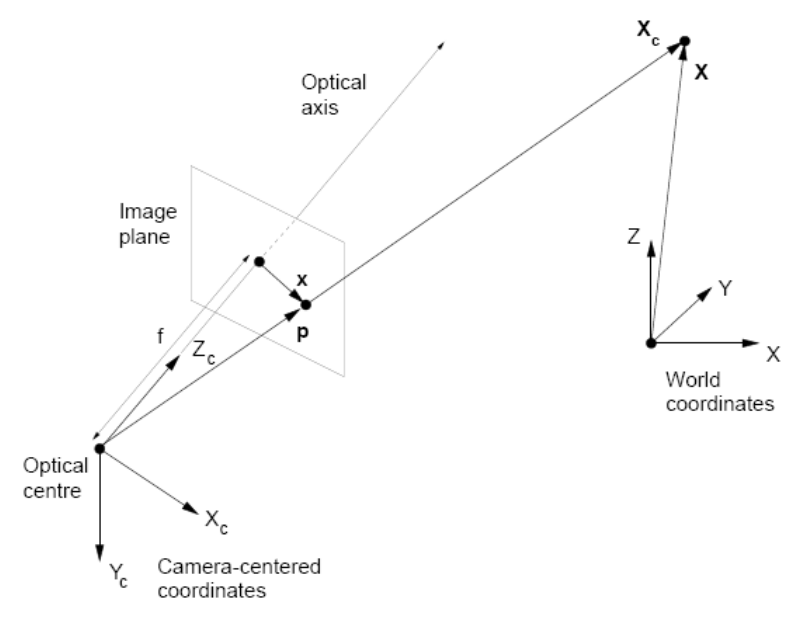
\includegraphics[width=5cm]{Figs/Introducao/cam_coord.png}}}
%     \end{center}
%     \caption{Localização e relação das coordenadas da câmera com a do mundo. Fonte~\cite{FergusL1}.}
%     \label{fig:intro_cam_coord}
% \end{figure*}

A projeção $\mathbf{P}$ é a combinação de três transformações de coordenadas:~\emph{matriz de intrínsecos} $\mathbf{K}$ (posicionamento do ponto focal e do ponto principal, ângulo entre eixos e outros), matriz de projeção $[\mathbf{I} ~|~ \mathbf{0} ]$ e~\emph{matriz de extrínsecos} $[\mathbf{R} ~|~ \mathbf{t} ]$ (relação entre as coordenadas da câmera e os~\emph{pixels})~\cite{FergusL1}.

% , onde:
% $$
%     {\mathbf{K}}
%     =
%     \begin{bmatrix} 
%         f_x & \alpha & c_x\\
%         0 & f_y & c_y \\
%         0 & 0 & 1 \\
%     \end{bmatrix}
%     =
%     \begin{bmatrix} 
%         \text{dist. focal em~\emph{pixels} hor.} & \text{âng. entre eixos} & \text{centro hor.} \\
%         0 & \text{dist. focal em~\emph{pixels} ver.} & \text{centro ver.} \\
%         0 & 0 & 1 \\
%     \end{bmatrix}
%     .
% $$

\subsection{Visão Estéreo}
    \label{subsec:intro_stereo}
A partir de duas ou mais imagens de um mesmo local (objeto ou até uma pessoa), é possível extrair, identificar e triangular suas características nas imagens e obter uma modelagem 3D; os problemas de~\emph{correspondência}~\cite{FergusL1}.

A priori a busca pelas correspondências ocorreria por toda a imagem; com uso das~\emph{linhas epipolares} reduz-se a uma busca linear. 
% Com base na Figura~\ref{fig:intro_stereo_epipolar_exemplo}, sabe-se
Sabe-se
que o ponto real $\mathbf{p}$ é representado pelos pontos $\mathbf{x_0}$ e $\mathbf{x_1}$ das imagens. Ao reprojetar linearmente o ponto $\mathbf{p}$ no infinito, $\mathbf{p_{\infty}}$, de modo a continuar sendo projetado no ponto $\mathbf{x_0}$ é possível determinar a linha epipolar a partir da diferença de projeção em relação a $\mathbf{x_1}$~\cite{Szeliski2012}.

% \begin{figure*}[!ht]
%     \begin{center}
%         \bmvaHangBox{\fbox{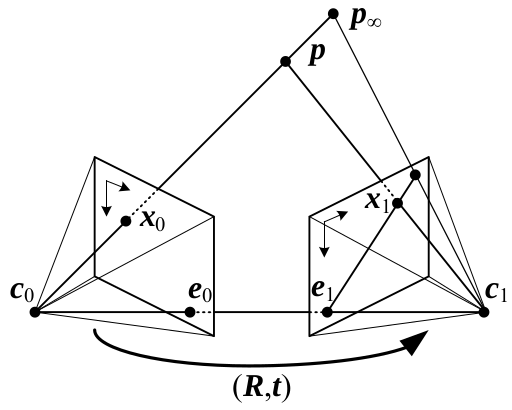
\includegraphics[width=3.8cm]{Figs/Introducao/linha_epipolar.png}}}
%     \end{center}
%     \caption{Representação visual da determinação de uma linha epipolar. Fonte~\cite{Szeliski2012}.}
%     \label{fig:intro_stereo_epipolar_exemplo}
% \end{figure*}

Com a aquisição das linhas epipolares de imagens correspondentes é possível reduzir a busca de correspondência numa linha horizontal, para alguns conjuntos de imagem~\cite{Szeliski2012}, 
% conforme ilustrado na Figura~\ref{fig:intro_stereo_match},
sendo denominado de~\emph{retificação}.

% \begin{figure}[!ht]
%     \centering
%     \begin{tabular}{cc}
%         \bmvaHangBox{\fbox{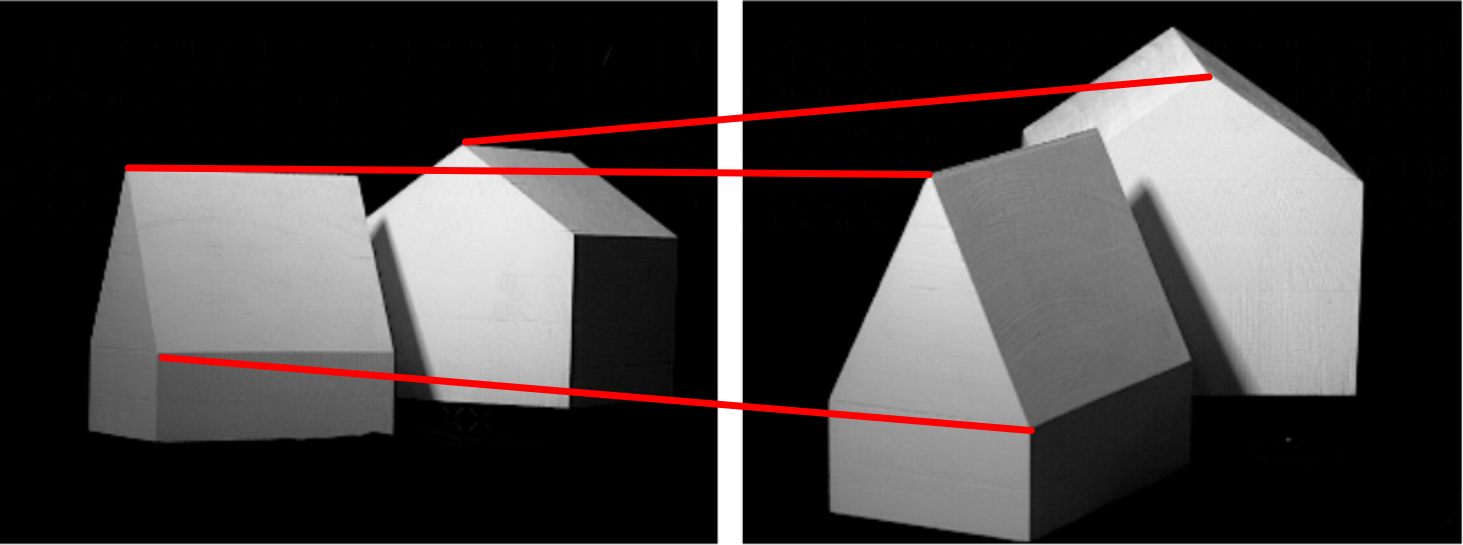
\includegraphics[height=1.5cm]{Figs/Introducao/original_stereo_.png}}}&
%         \bmvaHangBox{\fbox{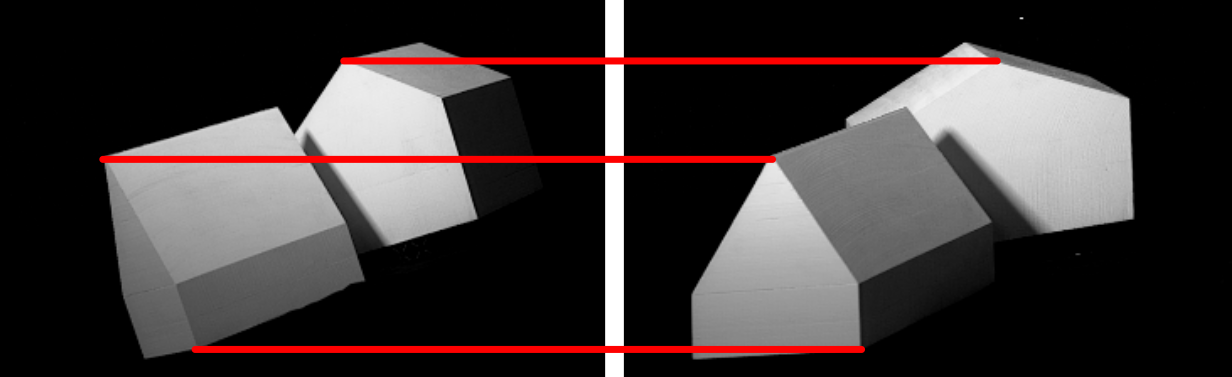
\includegraphics[height=1.5cm]{Figs/Introducao/ret_stereo_.png}}}\\
%         (a)&(b)
%     \end{tabular}
%     \caption{Retificação de um par de imagens estéreo, onde (a) são as imagens originais com linhas epipolares em diversas direções e (b) são as imagens retificação com todas as linhas epipolares na horizontal. Adaptado~\cite{Lazebnik1}.}
%     \label{fig:intro_stereo_match}
% \end{figure}

Além disso, a partir de duas imagens correspondentes a quantidade de movimentação que é percebida é denominada~\emph{disparidade}. Essa grandeza informa a distância entre os~\emph{pixels} correspondentes das imagens: $d_{(x, y)} = |x - x'| + |y - y'|$. Ao se calcular a disparidade para todos os~\emph{pixels} da imagem obtém-se seu~\emph{mapa de disparidade}
% , conforme ilustrado na Figura~\ref{fig:intro_stereo_disp_exemplo}
. No cenário de imagens correspondentes retificadas onde uma está certamente à direita da outra, a busca é ainda reduzida à esquerda do~\emph{pixel} base e vice-versa.

% \begin{figure}[!ht]
%     \centering
%     \begin{tabular}{cccc}
%         \bmvaHangBox{\fbox{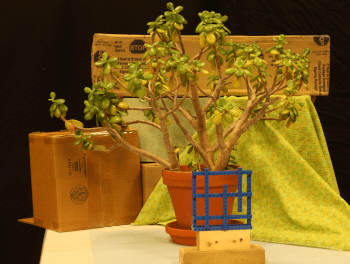
\includegraphics[width=3.3cm]{Figs/Introducao/exemplo_left.png}}}&
%         \bmvaHangBox{\fbox{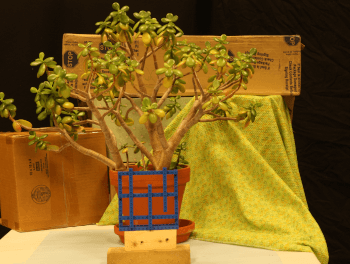
\includegraphics[width=3.3cm]{Figs/Introducao/exemplo_right.png}}}&
%         \bmvaHangBox{\fbox{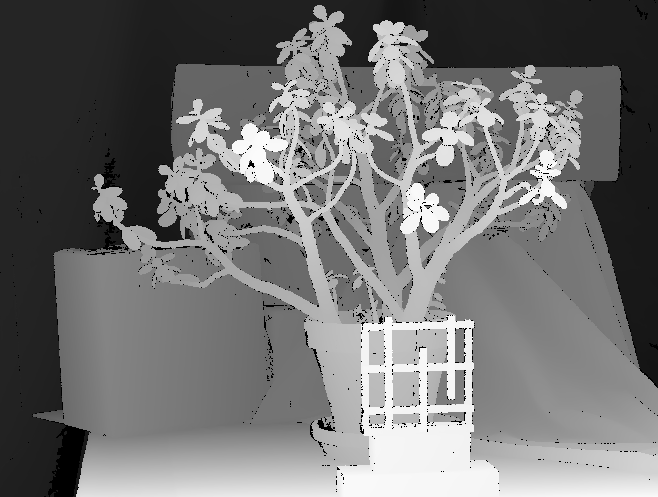
\includegraphics[width=3.3cm]{Figs/Introducao/exemplo_gt.png}}}\\
%         (a)&(b)&(c)
%     \end{tabular}
%     \caption{Mapa de disparidade para um par de imagens correspondentes retificadas, com as imagens exploradas por este trabalho. Têm-se os três componentes para esse mapa: (a) imagem base, (b) imagem correspondente à imagem base e (c) mapa de disparidade da imagem base.}
%     \label{fig:intro_stereo_disp_exemplo}
% \end{figure}

Com a aquisição do mapa de disparidade e em pose dos dados das câmeras (distância focal da imagem base $f$ e distância do mundo entre as câmeras $b$) é possível calcular o~\emph{mapa de profundidade}, uma vez que $Z_{xy} = (f \cdot b) /d_{xy}$.

\section{Desafio}
    \label{sec:desa}
Ao utilizar pares de imagens correspondentes deve-se buscar o entendimento e a exploração sobre a visão estéreo ao: extrair mapas de disparidade e de profundidade; utilizar os dados de calibração das câmeras e medição de objetos em 3D. Para tanto, três requisitos devem ser atendidos:

\begin{enumerate}
    \item \textbf{Estimativa de mapa de profundidade a partir de imagens estéreo retificadas}: manipulando, pelo menos, os conjuntos de  imagens~\emph{``Jadeplant''} e~\emph{``Playtable''} da base de imagens de~\emph{Middleburry} de $2014$~\cite{Middleburry2014} da configuração perfeita para computar os mapas de disparidade e de profundidade; a métrica BAD2.0 deve ser empregada;
    \item \textbf{Câmeras estéreo com convergência}: manipulando, pelo menos, os conjuntos de imagens~\emph{``Morpheus''} não retificado da base de imagens produzida por Furukawa e Ponce (indisponível) para computar o mapa de disparidade;
    \item \textbf{Paralelepípedo}: manipulando os mapas obtidos com o requisito anterior para computar a menor caixa que comporta os cliques de mouse fornecidos.
\end{enumerate}

\section{Metodologia}
    \label{sec:met}
A implementação foi realizada em Python, ver. $3.7.2$, utilizando~\emph{OpenCV} e está disponível online no GitHub~\cite{codigo2020}.

Com o intuito de intensificar a caracterização dos~\emph{pixels} das imagens de entradas, estas são convertidas para a escala de cinza e têm seu contraste e brilho ajustados seguidos pela equalização de histograma, conforme demonstrado na Figura~\ref{fig:met_pre_process}.

\begin{figure}[!ht]
    \centering
    \begin{tabular}{ccc}
        \bmvaHangBox{\fbox{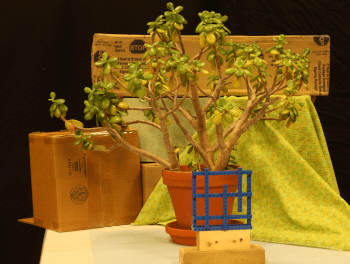
\includegraphics[width=3.6cm]{Figs/Introducao/exemplo_left.png}}}&
        \bmvaHangBox{\fbox{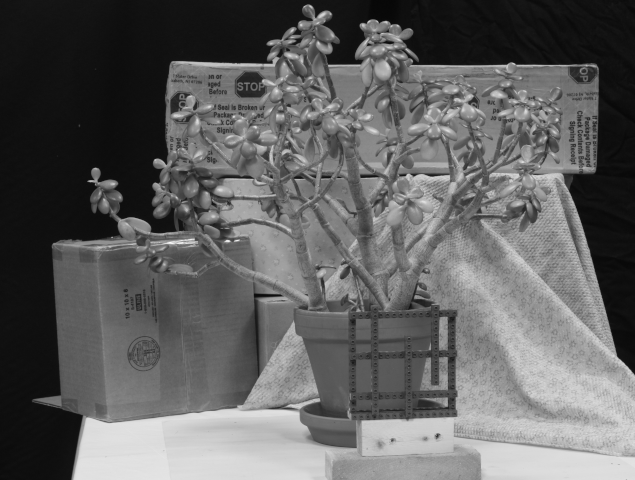
\includegraphics[width=3.6cm]{Figs/Metodologia/esq_480x635.png}}}&
        \bmvaHangBox{\fbox{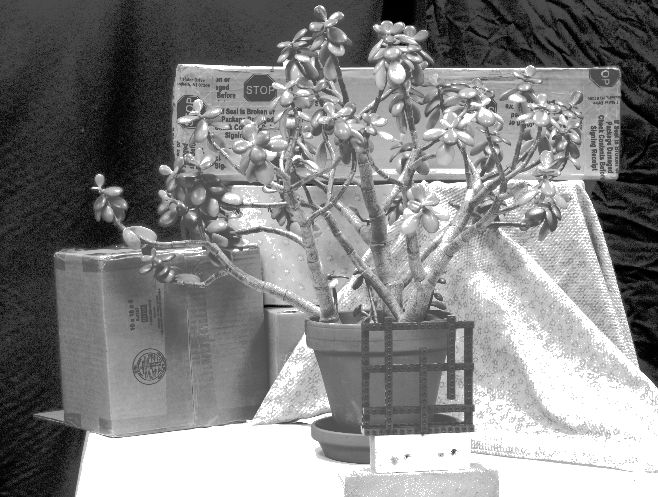
\includegraphics[width=3.6cm]{Figs/Metodologia/gray_left.png}}}\\
        (a)&(b)&(c)
    \end{tabular}
    \caption{Evolução do pré-processamento das imagens base, onde esta (a) é convertida para escala de cinza (b) e é ajustada (c).}
    \label{fig:met_pre_process}
\end{figure}

Com o caráter exploratório como principal objetivo, cinco algoritmos foram implementados:

\begin{enumerate}
    \item \textbf{OpenCV (OCV)}: método do algoritmo SBGM (\emph{Semi-Global Block Matching}) implementados pela biblioteca, gerando dois mapas de disparidades tendo ambas as imagens como base e pós-processando-os por intermédio da filtragem WLS (\emph{Weighted Least Squares}). Para tanto, uma exploração sobre a parametrização também foi realizada:~\emph{uniquenessRatio} (porcentagem de vantagem entre as duas melhores correspondências para sua confirmação),~\emph{speckleWindowSize} (tamanho máximo das regiões de disparidade suavizadas),~\emph{speckleRange} (variação máxima entre os componentes conectados),~\emph{wls\_lambda} (quantidade de regularização durante o filtro) e~\emph{wls\_sigma\_color} (sensibilidade às bordas durante a filtragmem);
    \item \textbf{Busca linear (BL)}: em cada linha retificada, considera-se como referência $\mathbf{R}$ (imagem da esquerda) um vetor de tamanho máximo $N$ e como janela de busca (imagem da direita) de tamanho máximo $M$. Com isso desliza-se uma janela do tamanho da referência obtida e a diferença entre janela deslizante $\mathbf{W}$ e a referência é computada, seguida pela busca da janela de menor diferença. A janela encontrada é validada considerando uma variação $|V|/\text{\emph{pixel}}$;
    \item \textbf{Correlação cruzada (CC)}: semelhante à~\emph{Busca linear} até o cálculo da diferença, visto que é computado ``o ângulo'' entre a janela deslizante e a referência: $(\mathbf{R} \cdot \mathbf{W})/(|\mathbf{R}| \cdot |\mathbf{W}|)$. A janela encontrada é validada considerando uma variação menor ou igual a $30º$ ($0,15$);
    \item \textbf{Janela deslizante (JD)}: semelhante à~\emph{Busca linear}, considera uma vizinhança 2D quadrada de tamanho fixo;
    \item \textbf{Janela deslizante adaptativa (JDA)}: semelhante à~\emph{Janela deslizante}, considera uma vizinhança 2D de tamanho variável controlada pela janela de busca.
\end{enumerate}

Ainda sob esta perspectiva, foram explorados diversos tamanhos ímpares para os blocos de verificação com $N \in [3, 17]$. Além disso, tanto os mapas de disparidade e de profundidade foram normalizados para comparação também.

\section{Resultados}
    \label{sec:result}
Considerando o aspecto exploratório deste projeto sobre visão estéreo, as primeiras investigações manipularam as imagens redimensionadas, devido à limitação do tempo de processamento.

A avaliação sobre os parâmetros do algoritmo~\emph{OpenCV} se deu como: $\text{\emph{wls\_sigma\_color}} \in [80, 7980] \implies 80$, $\text{\emph{wls\_lambda}} \in [0.5, 1.5] \implies 0.5$, uma vez que os erros foram diretamente proporcionais às suas variações; $\text{\emph{speckleRange}} \in [1, 2] \implies 1$, $\text{\emph{speckleWindowSize}} \in [50, 200] \implies 200$, $\text{\emph{uniquenessRatio}} \in [5, 15] \implies 10$, uma vez que não demonstraram influência direta frente os demais parâmetros. Com esta análise realizada, têm-se os resultados por requisitos.

\subsection{Requisito 1}
    \label{subsec:result_req1}
Devido à pouca fluência sobre a biblioteca~\emph{NumPy} este foi o requisito mais desafiador, já que a abordagem de manipulação das imagens comumente utilizada nas linguagens C/C++ foi utilizada: uso de laços~\emph{for}, o que tem baixíssima performance em Python.

Uma vez utilizando a biblioteca, os algoritmos foram avaliados tanto no original quanto normalizados, com exceção da~\emph{Janela Deslizante Adaptativa} por ser um algoritmo de baixa performance temporal. A Tabela~\ref{tab:result_req1_perf} traz os desempenhos sobre os dados originais, encontrando os melhores resultados para ambas as imagens base com a~\emph{Janela Deslizante} de tamanho $15$ e os piores com a~\emph{OpenCV} independente do tamanho da janela. Para os dados normalizados, a Tabela~\ref{tab:result_req1_perf_norm}, encontrando os melhores resultados para ambas as imagens com a~\emph{OpenCV} variando o tamanho entre $9-11$ e os piores com a~\emph{Busca Linear} para ``Jadeplant'' e com a~\emph{Correlação Cruzada} para ``Playtable'' ambas com janelas de tamanho $5$.

\begin{table}[!ht]
    \centering
    \small
    \begin{tabular}{c|c|c|c|c|c|c|c|c}
        \cline{3-9}
        \multicolumn{2}{l}{} & \multicolumn{7}{c}{Tamanho do bloco, $N$} \\ \hline
        Algoritmo & Imagem & 3 & 5 & 7 & 9 & 11 & 13 & 15 \\ \hline
        \multirow{2}{*}{OCV} & Jadeplant & \textcolor{violet}{$0.0$} & $0.0$ & $0.0$ & $0.0$ & $0.0$ & $0.0$ & $0.0$ \\ \cline{2-9}
         & Playtable & \textcolor{violet}{$0.0$} & $0.0$ & $0.0$ & $0.0$ & $0.0$ & $0.0$ & $0.0$ \\ \hline
        \multirow{2}{*}{BL} & Jadeplant & $0.62$ & $0.81$ & $0.72$ & $0.88$ & $1.41$ & $0.59$ & $0.55$ \\ \cline{2-9}
         & Playtable & $1.84$ & $0.75$ & $0.78$ & $1.53$ & $1.37$ & $1.46$ & $1.39$ \\ \hline
        \multirow{2}{*}{CC} & Jadeplant & $1.01$ & $1.08$ & $0.95$ & $0.9$ & $0.89$ & $0.88$ & $0.86$ \\ \cline{2-9}
         & Playtable & $3.41$ & $5$ & $1.32$ & $0.93$ & $0.79$ & $0.72$ & $0.68$ \\ \hline
        \multirow{2}{*}{JD} & Jadeplant & $2.33$ & $3.29$ & $4.18$ & $5.04$ & $5.89$ & $6.74$ & \textcolor{teal}{$7.56$} \\ \cline{2-9}
         & Playtable & $31.56$ & $40.74$ & $45.12$ & $47.84$ & $49.55$ & $50.76$ & \textcolor{teal}{$51.66$} \\ \hline
        \multirow{2}{*}{JDA} & Jadeplant & - & $2.62$ & - & - & - & - & - \\ \cline{2-9}
         & Playtable & - & - & - & - & - & - & - \\ \hline
    \end{tabular}
    \caption{Desempenho percentual dos acertos dos algoritmos com base na métrica BAD2.0.}
    \label{tab:result_req1_perf}
\end{table}

\begin{table}[!ht]
    \centering
    \small
    \begin{tabular}{c|c|c|c|c|c|c|c|c}
        \cline{3-9}
        \multicolumn{2}{l}{} & \multicolumn{7}{c}{Tamanho do bloco, $N$} \\ \hline
        Algoritmo & Imagem & 3 & 5 & 7 & 9 & 11 & 13 & 15 \\ \hline
        \multirow{2}{*}{OCV} & Jadeplant & $8.47$ & $9.15$ & $12.47$ & $46.66$ & \textcolor{teal}{$52.13$} & $51.31$ & $50.22$ \\ \cline{2-9}
         & Playtable & $4.65$ & $4.66$ & $4.68$ & \textcolor{teal}{$55.85$} & $54.92$ & $54.85$ & $53.77$ \\ \hline
        \multirow{2}{*}{BL} & Jadeplant & $4.47$ & $4.09$ & $3.93$ & $4.04$ & $4.12$ & $4.25$ & $4.36$ \\ \cline{2-9}
         & Playtable & $4.53$ & \textcolor{violet}{$4.05$} & $4.13$ & $5.25$ & $5.11$ & $4.87$ & $4.75$ \\ \hline
        \multirow{2}{*}{CC} & Jadeplant & $3.75$ & \textcolor{violet}{$3.64$} & $3.7$ & $3.82$ & $3.9$ & $3.93$ & $3.98$ \\ \cline{2-9}
         & Playtable & $5.29$ & $8.86$ & $17.3$ & $29.53$ & $38.64$ & $39.47$ & $36.86$ \\ \hline
        \multirow{2}{*}{JD} & Jadeplant & $4.13$ & $4.07$ & $4.04$ & $4$ & $3.97$ & $3.95$ & $3.94$ \\ \cline{2-9}
         & Playtable & $8.07$ & $7.68$ & $7.71$ & $7.76$ & $7.84$ & $7.91$ & $7.96$ \\ \hline
        \multirow{2}{*}{JDA} & Jadeplant & - & - & - & - & - & - & - \\ \cline{2-9}
         & Playtable & - & - & - & - & - & - & - \\ \hline
    \end{tabular}
    \caption{Desempenho percentual dos acertos dos algoritmos normalizados com base na métrica BAD2.0.}
    \label{tab:result_req1_perf_norm}
\end{table}

A partir da Figura~\ref{fig:result_req1_disp_map} fica claro o motivo da~\emph{OpenCV} ficar com os piores resultados: os valores ficaram em um~\emph{range} muito superior ao esperado ($[-30000, 10000]$ frente ao $[27, 600]$, para a ``Jadeplant'' e $[0, 4000+]$ frente ao $[27, 270]$, para a ``Playtable''); o mesmo não pode ser dito sobre os melhores. Para estes últimos, a grande quantidade de detalhes da ``Jadeplant'' não foi bem administrada pelos algoritmos, uma vez que nenhum teve um aproveitamento acima de $10\%$, mas como a ``Playtable'' possui regiões mais constantes os algoritmos tiveram melhores desempenhos. Ao passo que ao normalizar os resultados no~\emph{range} $[0, 255]$, como ilustrados na Figura~\ref{fig:result_req1_disp_map_norm}, o algoritmo da~\emph{OpenCV} detêm os melhores resultados por possuir os blocos correspondentes mais bem definidos e na mesma faixa do~\emph{groun truth} normalizado.

\begin{figure}[!ht]
    \centering
    \begin{tabular}{cc}
        \bmvaHangBox{\fbox{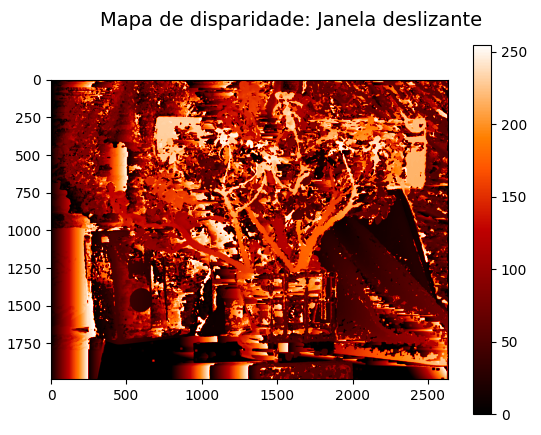
\includegraphics[width=5cm]{Figs/Resultados/jd_windowing_disp_map_bl15.png}}}&
        \bmvaHangBox{\fbox{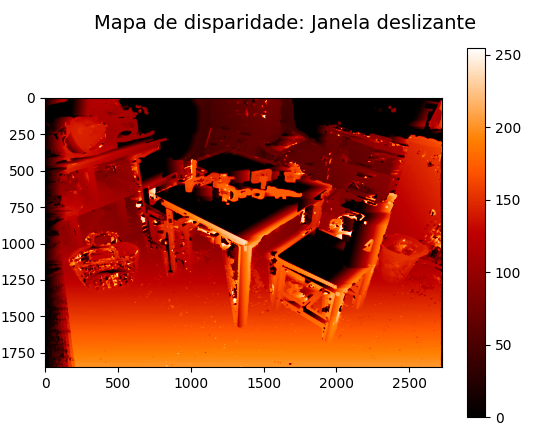
\includegraphics[width=5cm]{Figs/Resultados/pt_windowing_disp_map_bl15.png}}}\\
        (a)&(b) \\
        \bmvaHangBox{\fbox{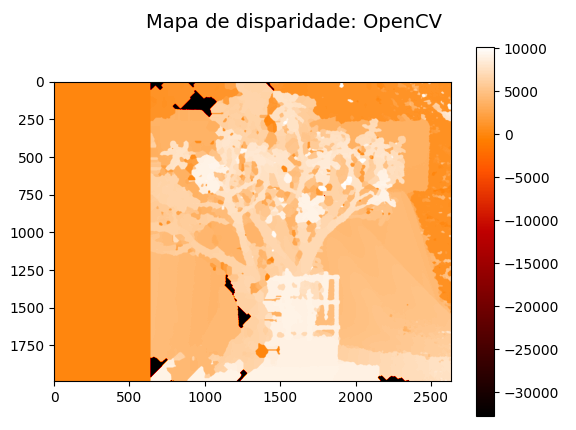
\includegraphics[width=5cm]{Figs/Resultados/jd_basic_disp_map_bl3.png}}}&
        \bmvaHangBox{\fbox{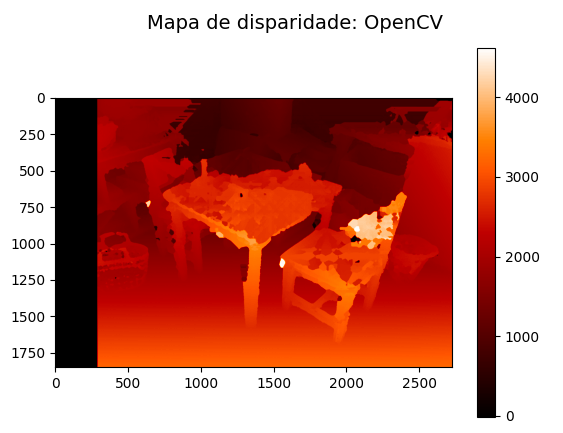
\includegraphics[width=5cm]{Figs/Resultados/pt_basic_disp_map_bl3.png}}}\\
        (c)&(d)
    \end{tabular}
    \caption{Mapas de disparidade dos melhores e piores resultados, onde (a) e (c) são o melhor e o pior, respectivamente, para ``Jadeplant'' e (b) e (d) para ``Playtable''.}
    \label{fig:result_req1_disp_map}
\end{figure}

\begin{figure}[!ht]
    \centering
    \begin{tabular}{cc}
        \bmvaHangBox{\fbox{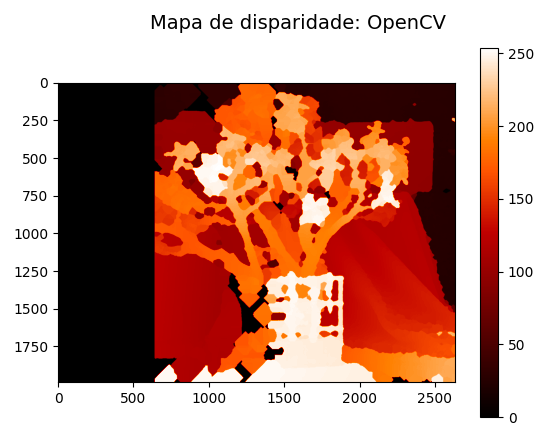
\includegraphics[width=5cm]{Figs/Resultados/eq_jd_basic_disp_map_bl11.png}}}&
        \bmvaHangBox{\fbox{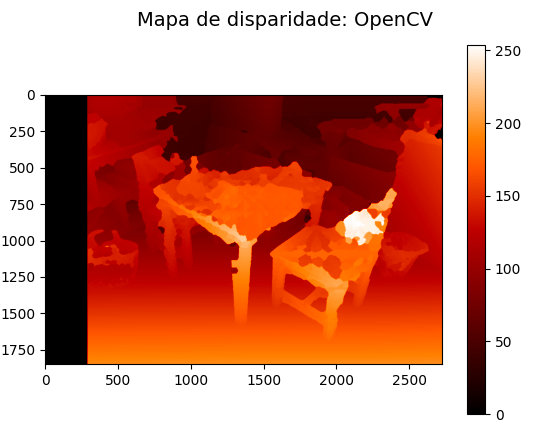
\includegraphics[width=5cm]{Figs/Resultados/eq_pt_basic_disp_map_bl9.png}}}\\
        (a)&(b) \\
        \bmvaHangBox{\fbox{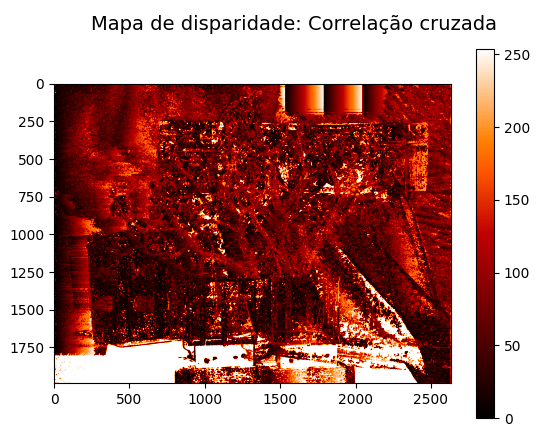
\includegraphics[width=5cm]{Figs/Resultados/eq_jd_x_correlation_disp_map_bl5.png}}}&
        \bmvaHangBox{\fbox{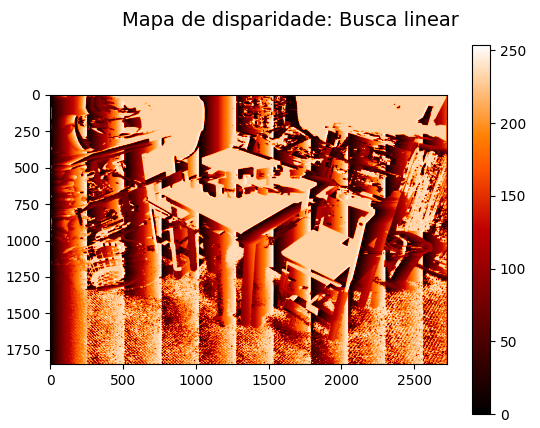
\includegraphics[width=5cm]{Figs/Resultados/eq_pt_linear_search_disp_map_bl5.png}}}\\
        (c)&(d)
    \end{tabular}
    \caption{Mapas de disparidade normalizados dos melhores e piores resultados, onde (a) e (c) são o melhor e o pior, respectivamente, para ``Jadeplant'' e (b) e (d) para ``Playtable''.}
    \label{fig:result_req1_disp_map_norm}
\end{figure}

Na análise sobre os mapas de profundidade, os erros nos cálculos dos mapas de disparidade tornam-se mais evidentes, já que a Figura~\ref{fig:result_req1_depth_map} demonstram-os como imagens de valor único e de baixíssima profundidade, ou seja, simplesmente errados. Com base nos dados das câmeras, a variação de profundidade deveria estar entre $4,63$ ($d_{xy}=600$) e $102,99$ ($d_{xy}=27$) metros para a ``Jadeplant'' e entre $1,67$ ($d_{xy}=270$) e $16,65$ ($d_{xy}=27$) para a ``Playtable''.

\begin{figure}[!ht]
    \centering
    \begin{tabular}{cc}
        \bmvaHangBox{\fbox{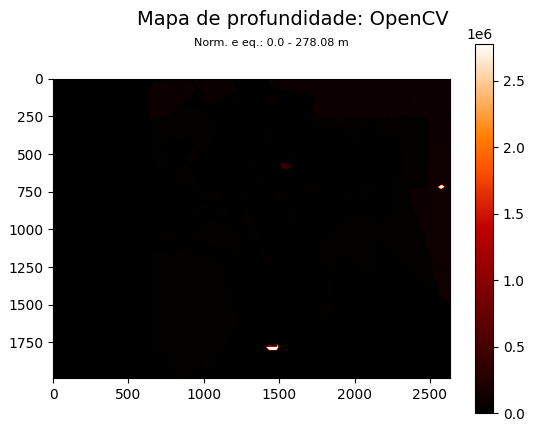
\includegraphics[height=4.5cm]{Figs/Resultados/eq_jd_dp_basic_disp_map_eq_bl11.png}}}&
        \bmvaHangBox{\fbox{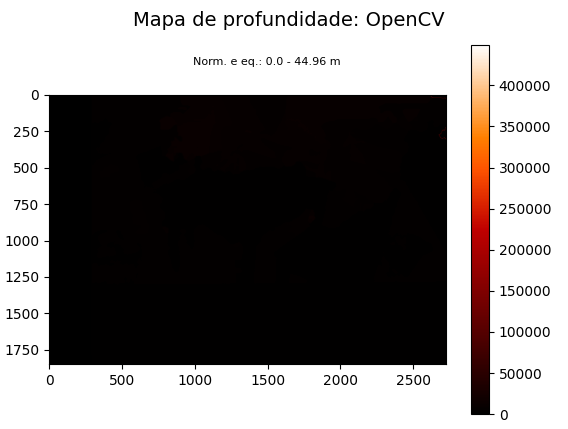
\includegraphics[height=4.5cm]{Figs/Resultados/eq_pt_dp_basic_disp_map_eq_bl9.png}}}\\
        (a)&(b)
    \end{tabular}
    \caption{Mapas de profundidade para os mapas de disparidade com as melhores taxas de acertos, onde (a) é o melhor para a ``Jadeplant'' e (b) para ``Playtable''.}
    \label{fig:result_req1_depth_map}
\end{figure}

\subsection{Requisito 2}
    \label{subsec:result_req2}
Com base nos resultados do Requisito~\ref{subsec:result_req1} e considerando que: (a) não há uma base para comparação e (b) as imagens não estão necessariamente retificadas; o algoritmo~\emph{Janela Deslizante} com blocos de tamanho $15$ foi selecionado para este requisito. Dessa forma, a exploração aconteceu sobre o tamanho da janela de busca $M \in [100, 800]$, por também ser desconhecida para esta base.

Com isso, os mapas de disparidade não apresentaram bons resultados visuais, uma vez que não é possível vislumbrar uma similaridade com as imagens originais, como demonstrado na Figura~\ref{fig:result_req2_disp_map}. Com o intuito de melhorar o desempenho, as imagens correspondes tiveram o mesmo pré-processamento das imagens do primeiro requisito, sendo realizada uma busca pelos ponto-chaves e suas correspondências entre as imagens, com a finalidade de identificar as linhas epipolares, seguida pela retificação das imagens considerando as suas próprias homografias.

\begin{figure}[!ht]
    \centering
    \begin{tabular}{ccc}
        \bmvaHangBox{\fbox{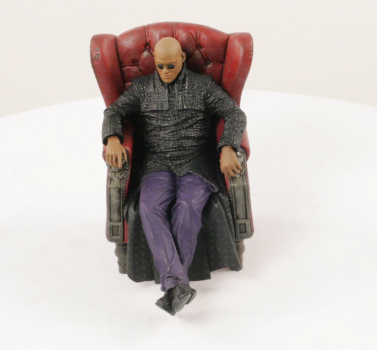
\includegraphics[width=3.5cm]{Figs/Resultados/MorpheusL_rsz.jpg}}}&
        \bmvaHangBox{\fbox{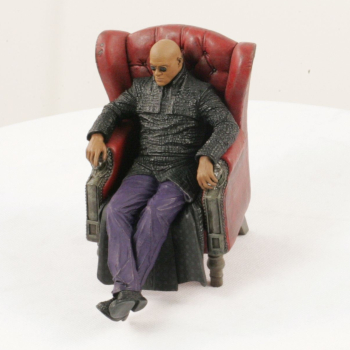
\includegraphics[width=3.5cm]{Figs/Resultados/MorpheusR_rsz.jpg}}}&
        \bmvaHangBox{\fbox{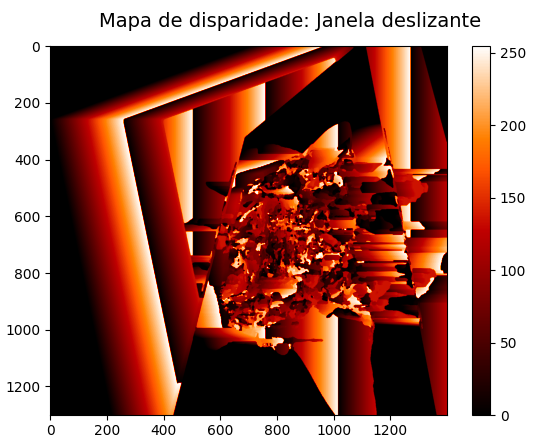
\includegraphics[width=3.5cm]{Figs/Resultados/morpheus_lk400.png}}}\\
        (a)&(b)&(c) \\
        \bmvaHangBox{\fbox{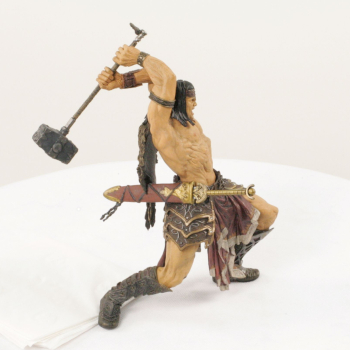
\includegraphics[width=3.5cm]{Figs/Resultados/warriorL_rsz.jpg}}}&
        \bmvaHangBox{\fbox{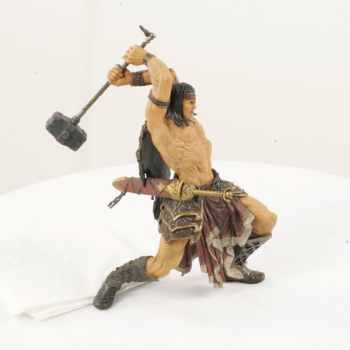
\includegraphics[width=3.5cm]{Figs/Resultados/warriorR_rsz.jpg}}}&
        \bmvaHangBox{\fbox{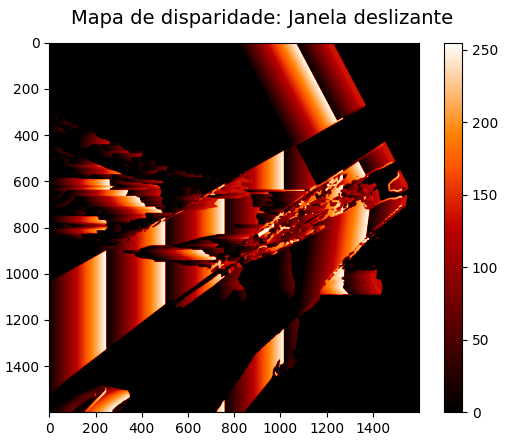
\includegraphics[width=3.5cm]{Figs/Resultados/warrior_lk400.png}}}\\
        (d)&(e)&(f)
    \end{tabular}
    \caption{Mapas de disparidade para o Requisito~\ref{subsec:result_req2}, onde (a) e (d) são as imagens base, (b) e (e) são as imagens correspondentes e (c) e (f) os mapas de disparidade com uma busca de até $400$~\emph{pixels} calculados para o ``Morpheus'' e ``Warrior'', respectivamente. Fonte das imagens (a), (b), (d) e (e) para a base de imagens desativada supracitada.}
    \label{fig:result_req2_disp_map}
\end{figure}



\subsection{Requisito 3}
    \label{subsec:result_req3}
Devido à falta de clareza e distinção dos resultados do Requisito~\ref{subsec:result_req2} não houve tentativa de desenvolvimento para este requisito.


\section{Conclusão}
    \label{sec:conc}
Os algoritmos implementados se provaram desafiadores seja pela dificuldade da programação seja por fatores intrínsecos. Para o Requisito~\ref{subsec:result_req1}, o algoritmo~\emph{OpenCV} apresentou os melhores resultados visuais, por ter conseguido conectar os blocos relacionados, mas os valores de disparidade destoam do~\emph{ground truth}, o que justifica o seu baixo desempenho. Entretanto, ao normalizar os mapas de disparidade a taxa de acertos aumentou, justamente pela compactação das escalas distintas numa comum o que aumenta o número de boas ``colisões'' de disparidade, esta pode ser uma boa técnica a ser utilizada para quando os limites de disparidade são previamente conhecidos, como no caso em questão, pois poderiam ser escalonados à faixa conhecida.

Ao se deparar com o Requisito~\ref{subsec:result_req2}, entretanto, houve a constatação da fragilidade dos algoritmos desenvolvidos, sem considerar as influências do pré-processamento das imagens, devido a falta de solução para o problema apresentado.

\bibliography{refs}

\end{document}
